\documentclass[./main.tex]{subfiles}
\begin{document}

En el capítulo anterior 
En las secciones anteriores observamos que el modelo de fase con bifurcación de ciclo infinito y ruido blanco gaussiano con una amplitud de modulación mayor a la frecuencia del uniforme puede dar lugar a actividad pulsátil. Esta actividad pulsátil es producto de perturbaciones que genera el ruido en el régimen excitable. Estudiamos que, en estas condiciones, los valores de ruido regulan la coherencia de esta actividad pulsátil. Por otro lado, cuando la amplitud de modulación es menor que la frecuencia del uniforme, el ruido desordena las oscilaciones. Estas características convierten a este modelo teórico en un candidato interesante para describir las oscilaciones intermitentes. Sin embargo, observamos que las propiedades dinámicas de la fase, como la duración de pulsos, dependen de los parámetros del modelo de una manera no trivial.  

En este marco, en esta sección nos preguntamos qué capacidad tiene el modelo de fase con bifurcación de ciclo infinito y ruido blanco gaussiano de reproducir las oscilaciones intermitentes de la dinámica de actividad de ERK en ESCs. Comenzamos por analizar la posibilidad que el modelo teórico ajuste a observables calculados sobre los datos experimentales. Elegimos observables simples y que resumen muchas de las principales características de la dinámica de activación de ERK en ESCs, y comparamos su estadística calculada sobre el modelo teórico con la de nuestros datos experimentales. De esta manera, buscamos entender si las propiedades dinámicas de la descripción teórica son compatibles con nuestras observaciones experimentales. En segundo lugar, diseñamos un protocolo para ajustar de manera sistemática los observables calculados sobre el modelo teórico a los calculados sobre los experimentos. A partir de esta calibración, evaluamos qué magnitudes dinámicas que describen las oscilaciones intermitentes en nuestras observaciones experimentales puede reproducir el modelo.



Buscamos describir las oscilaciones intermitentes de la dinámica de activación de ERK en ESCs, donde intervalos oscilatorios se intercalan con intervalos de silencio y pulsos aislados, con un modelo matemático de baja dimensionalidad. En el capítulo anterior encontramos que un modelo de fase con bifurcación de ciclo infinito y ruido blanco gaussiano aditivo es capaz de ajustar la estadística de la duración de pulsos, el intervalo de interpulsado y la tasa de pulsado, observables simples que resumen características importantes de las mediciones experimentales. A partir de este ajuste, este modelo teórico puede reproducir la proporción promedio de que los datos experimentales pulsaban, así como la cantidad de pulsos totales que observamos en los experimentos. Además, puede dar lugar tanto a pulsos aislados, como pulsos consecutivos organizados en trenes. 

Si bien este panorama es alentador, observamos que el modelo falla en reproducir la heterogeneidad de actividad que observamos en los datos experimentales. Nuestras observaciones sugieren que este modelo es insuficiente para recapitular los casos límites de actividad pulsátil individual, en donde las células pulsaban durante toda la medición o no pulsaban nunca. Además, los pulsos suelen ser aislados o estar organizados en trenes cortos en comparación con nuestras observaciones. En resumen, el modelo de fase con bifurcación de ciclo infinito y ruido blanco gaussiano aditivo es insuficiente para describir las oscilaciones intermitentes de actividad de ERK en ESCs. 

Inspirados en estos resultados, en este capítulo proponemos modificaciones al modelo teórico con el que venimos trabajando para dar con una descripción teórica de las oscilaciones intermitentes de actividad de ERK que observamos en ESCs. Comenzamos por explorar la idea de que la actividad pulsátil de ERK pueda ser descripta a partir de transiciones entre el régimen oscilatorio y el excitable, que sin perturbaciones dará lugar a intervalos de silencio. Para esto, estudiamos los efectos de proponer variabilidad en la amplitud de modulación del modelo de fase con bifurcación de ciclo infinito, en donde estas variaciones estén reguladas con una escala temporal. En segundo lugar, integramos esta idea a la del capítulo anterior. Analizamos las capacidades y limitaciones de describir la dinámica de actividad de ERK como un sistema dinámico que simultáneamente de lugar a transiciones entre los regímenes dinámicos oscilatorio y excitable, y tenga perturbaciones capaces de generar actividad pulsátil en el excitable. Para terminar, evaluamos si la variabilidad en la amplitud de modulación puede ser descripta como un proceso estacionario, y no un proceso que varíe durante cada medición como hipotetizamos en los dos casos anteriores.  


\section{Variabilidad en la amplitud de modulación como reguladora de la actividad pulsátil heterogénea}
\label{C7_sec:OU}
\sectionmark{Variabilidad en la amplitud de modulación}

%motivación
Que en el ajuste del capítulo anterior hayamos logrado reproducir los valores intermedios de actividad que medimos en el experimento, pero hayamos observado una actividad pulsátil más homogénea nos sugiere que esta heterogeneidad pueda ser representada incorporando variabilidad de alguno de los parámetros del modelo. Por otro lado, los resultados del capítulo anterior nos muestran que para reproducir las oscilaciones intermitentes no es suficiente describir al sistema dinámico en un régimen excitable, en donde la actividad pulsátil aparezca consecuencia de perturbar al sistema dinámico con ruido blanco gaussiano, ni tampoco en un régimen puramente oscilatorio, donde las oscilaciones estén desordenadas por el ruido. Observamos que en esta descripción los pulsos se organizan en trenes cortos o aislados, y conduce a subestimar la cantidad de pulsos aislados del experimento.


En esta sección exploramos la idea de que la actividad pulsátil de ERK pueda ser descripta a partir de transiciones entre el régimen oscilatorio y el excitable descriptos por el modelo de fase con bifurcación de ciclo infinito. Con estas transiciones, esperamos obtener trenes de pulsos de mayor longitud cuando el sistema se encuentre en el régimen oscilatorio, intercalados con intervalos de silencios en el régimen excitable sin perturbar. Generaremos estas transiciones a partir de contemplar variabilidad en la amplitud de modulación, en donde las variaciones sean reguladas con una escala temporal. Describiéndolas con un origen estocástico, esperamos obtener una actividad pulsátil más heterogénea a lo largo de la población. 


\subsection{La amplitud de modulación como proceso de \textit{Ornstein-Uhlenbeck}}

Proponemos modificar el modelo de fase con bifurcación de ciclo infinito de la ecuación \ref{C5_eq:adler_determinista} proponiendo que la amplitud de modulación fluctúe \emph{lentamente} a lo largo del tiempo
\begin{equation}
    \partial_t  \theta(t) = \omega + \alpha_{ou}(t) \sin{(\theta(t))}.
    \label{C7_eq:alpha_ou}
\end{equation}

Un proceso estocástico ampliamente utilizado que incorpora fluctuaciones gobernadas por una escala temporal es el ruido de \textit{Ornstein-Uhlenbeck} \cite{SanMiguel2000}. Para introducir las fluctuaciones, consideraremos a la amplitud de modulación como un proceso de \textit{Ornstein-Uhlenbeck} estacionario (OU), donde 
\begin{align}
    \partial_t  \alpha_{ou}(t) &= \frac{1}{\tau} (\alpha_0 - \alpha(t)) + \sqrt{\frac{2}{\tau}}\sigma \xi_w(t) \label{C7_eq:OU_langevin}\\
    \alpha_{ou}(0) &= \alpha_0.
\end{align}
Con esta definición, la estadística de la amplitud de modulación es
\begin{align}
    \langle \alpha_{ou}(t) \rangle_t &= \alpha_0 \\
    \langle \alpha_{ou}(t) \; \alpha(t^\prime) \rangle_t &= \sigma^2 e^{- \lvert t-t^\prime \rvert / \tau } \label{C7_eq:OU_corr}.
\end{align}

A diferencia del ruido blanco gaussiano aditivo con el que trabajamos en el capítulo anterior, en la ecuación \ref{C7_eq:OU_langevin} podemos ver que el ruido de OU tiene un término de \emph{drift} proporcional a la diferencia entre el valor medio y el valor actual de la amplitud de modulación $\alpha_0 - \alpha_{ou}(t)$. Enfocándonos solamente en este término, observamos que si el valor actual del proceso sobrepasa su valor medio, la derivada de la amplitud de modulación será negativa y $\alpha_{ou}(t)$ evolucionará decreciendo su valor. En cambio, si el valor actual del proceso es menor que $\alpha_0$, la derivada será positiva y el valor del proceso crecerá. Esta característica en donde el proceso tiende siempre a desviarse hacia el valor finito $\alpha_0$ se conoce como \emph{reversión hacia la media} (figura \ref{C7_fig:OU_alpha}). \marginpar{valor medio de\\ la amplitud de\\modulación} La variable $\alpha_0$ es el \textbf{valor medio de la amplitud de modulación} en el tiempo. Al igual que la amplitud de modulación del modelo \ref{C5_eq:adler_determinista}, tiene unidades de $\frac{1}{\text{tiempo}}$. Por simplicidad, consideraremos sólo valores positivos de $\alpha_0$.

\begin{figure}
    \centering
    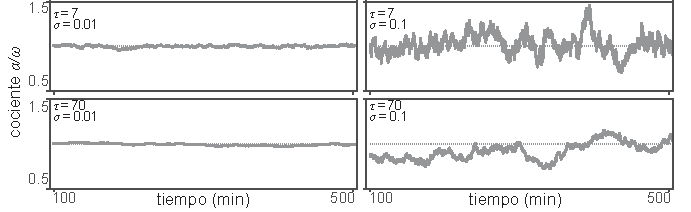
\includegraphics[width=1\columnwidth]{figures/chapter7/C7_OU_alpha.pdf} 
    \caption{\textbf{La amplitud de modulación como proceso de \textit{Ornstein-Uhlenbeck}}. Series temporales de la amplitud de modulación en función del tiempo para distintos valores de tiempo de reversión $\tau$ y volatilidad $\sigma$ indicados en el margen superior izquierdo de cada figura, en minutos y $1/\text{minutos}^{3/2}$ respectivamente. La amplitud de modulación se encuentra normalizada por una frecuencia $\omega$ constante. El valor medio de la amplitud de modulación $\alpha_0/\omega$ se encuentra representado con linea punteada. A modo de ejemplo, elegimos que el valor medio de la amplitud de modulación coincida con el punto donde aparece la bifurcación en el modelo de fase con bifurcación de ciclo infinito. Parámetros: $\alpha_0 = \frac{2\pi}{7 \text{ min}}$, $\omega = \frac{2\pi}{7 \text{ min}}$, $dt = 0.0001$, $d=10$ (apéndice \ref{C7_ap:OU_OUD_traces}).}
    \label{C7_fig:OU_alpha}
\end{figure} 

Continuando con el análisis del término de \textit{drift}, observemos que la velocidad de reversión no sólo depende de la diferencia entre el valor medio y el actual de la amplitud de modulación $\alpha_0 - \alpha(t)$, sino también la variable $\tau$.\marginpar{tiempo de\\reversión} El \textbf{tiempo de reversión} $\tau$ es la escala temporal con la que el proceso vuelve al valor medio (figura \ref{C7_fig:OU_alpha}).


Por otro lado, $\xi_w(t)$ en la ecuación \ref{C7_eq:OU_langevin} representa un proceso de ruido blanco gaussiano derivado de un proceso de \emph{Wiener}, que incorpora fluctuaciones instantaneas a la amplitud de modulación (ecuaciones \ref{C6_eq:wiener_mean},\ref{C6_eq:wiener_cov}).\marginpar{volatilidad} La \textbf{volatilidad} $\sigma$ es el factor de escala de este proceso $\xi_w(t)$, que modula cuán grandes son las fluctuaciones instantáneas  (figura \ref{C7_fig:OU_alpha}). Esta variable tiene unidades de $\frac{1}{\text{tiempo}^{3/2}}$, y consideraremos sólo valores positivos. 


La correlación temporal de la ecuación \ref{C7_eq:OU_corr} es no nula, y depende de el tiempo de reversión $\tau$ y la volatilidad cuadrada $\sigma^2$. Esto significa que los valores del ruido en diferentes momentos no son variables aleatorias independientes, sino que están correlacionadas. A este tipo de ruidos de correlación no nula se los suele llamar \emph{ruido de color}. El \emph{ruido blanco} con el que trabajamos en el capítulo anterior se recupera en el límite donde $\tau \rightarrow 0$ (descorrelacionado). 


%En términos sencillos, el proceso de \textit{Ornstein-Uhlenbeck} es un proceso que revierte a una media $\alpha_0$ en un tiempo promedio $\tau$ y volatilidad $\sigma$. %Es un proceso gaussiano, markoviano- pues cada instante futuro del proceso está determinado únicamente por su presente y no su pasado- y estacionario- la correlación de la ecuación \ref{C7_eq:OU_corr} no depende del tiempo-.


\subsection{Efectos del ruido de color en la amplitud de modulación sobre la fase}

En el capítulo \ref{ch4} observamos que variando la amplitud de modulación del modelo de fase con bifurcación de ciclo infinito es posible transicionar entre los regímenes oscilatorio y excitable. Esta transición ocurre en el punto de bifurcación, donde la amplitud de modulación es igual a la frecuencia del uniforme. Luego, si $\alpha < \omega$, nos encontramos con el régimen oscilatorio, y si $\alpha > \omega$, en el excitable. 

Proponer que la amplitud de modulación varíe en el tiempo conduce a la posibilidad de transicionar entre estos dos regímenes durante la evolución del proceso. En una serie temporal de la fase \xx(t), habrá momentos en donde $\alpha < \omega$ y la fase \xx(t) esté oscilando, y momentos donde el sistema se encuentre en el régimen excitable cuando $\alpha > \omega$ y la fase no esté oscilando. En la circunferencia trigonométrica de radio unidad, estas posibles transiciones entre los regímenes oscilatorio y excitable que producen las fluctuaciones de la amplitud de modulación se pueden interpretar como la creación, en caso de transicionar del oscilatorio hacia el excitable, o la colisión, en caso contrario, de los puntos fijos estables e inestable. En la señal, estas transiciones reflejarán combinaciones entre actividad pulsátil y silencios, como observamos en la figura \ref{C7_fig:OU_TS}.

\begin{figure}
    \centering
    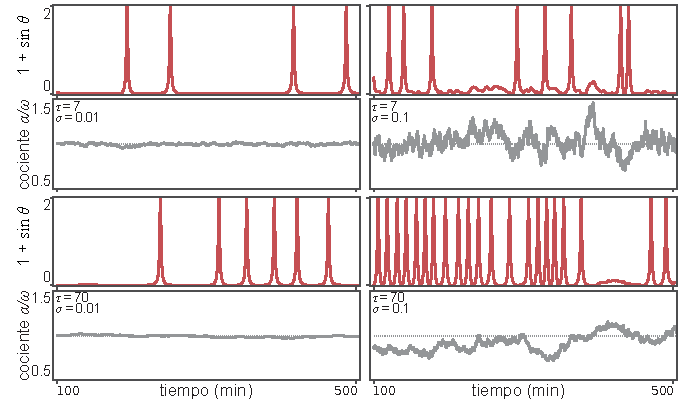
\includegraphics[width=1\columnwidth]{figures/chapter7/C7_OU_ex_traces.pdf} 
    \caption{\textbf{La amplitud de modulación como proceso de \textit{Ornstein-Uhlenbeck} conduce a transiciones entre los regímenes oscilatorio y excitable.}
    Arriba en rojo: señal de la fase del modelo \ref{C7_eq:alpha_ou} para distintos valores de tiempo de reversión $\tau$ y volatilidad $\sigma$, indicados en minutos y $1/\text{minutos}^{3/2}$ respectivamente. Abajo, en gris: la amplitud de modulación en función del tiempo correspondiente a cada señal. La amplitud de modulación se encuentra normalizada por la frecuencia frecuencia del uniforme $\omega$. El valor medio de la amplitud de modulación $\alpha_0/\omega$ se encuentra representado con linea punteada. Para ejemplificar, elegimos que el valor medio de la amplitud de modulación coincida con el punto donde aparece la bifurcación en el modelo de fase con bifurcación de ciclo infinito. Parámetros: $\alpha_0 = \frac{2\pi}{7 \text{ min}}$, $\omega = \frac{2\pi}{7 \text{ min}}$, $dt = 0.0001$, $d=10$ (apéndice \ref{C7_ap:OU_OUD_traces}).}
    \label{C7_fig:OU_TS}
\end{figure} 

Entonces, cuando la amplitud de modulación toma valores por debajo del punto de bifurcación, en la señal se traduce actividad pulsátil (línea gris por debajo de la línea punteada negra en la figura \ref{C7_fig:OU_TS}). En cambio, cuando tome valores por encima de este umbral, en señal se observará silenciosa (línea gris por encima de la línea punteada negra en la figura \ref{C7_fig:OU_TS}). En la figura \ref{C7_fig:OU_TS} observamos que el aumento del tiempo de reversión conduce trenes de pulsos más largos. Con la misma lógica, puede también conducir a silencios más largos. Por otro lado, el aumento de la volatilidad guía a que la amplitud de modulación fluctúe instantáneamente con mayor intensidad. Fluctuaciones de mayor intensidad dan lugar a una posibilidad mayor de atravesar por un corto lapso de tiempo la bifurcación, produciendo, por ejemplo, un pulso aislado o trenes de pulsos cortos.


Por otro lado, la frecuencia del uniforme determina cuán rápido se realiza una excursión de la fase que da lugar a un pulso. Además, $\alpha_0$ determinará cuán lejos se encuentra, en promedio, la amplitud de modulación de la bifurcación y por ende está asociado a qué características del proceso estocástico son necesarias para atravesarla. Por ejemplo, un valor de $\alpha_0$ lejano a la bifurcación dará lugar a menos transiciones entre regímenes que un valor cercano. En concreto, una volatilidad pequeña es suficiente para transicionar entre regímenes en casos donde $\alpha_0$ es cercano a $\omega$, pero no cuando es muy lejano. También, para un mismo tiempo de reversión, es probable que un sistema dinámico cuyo $\alpha_0$ es es cercano a $\omega$ pase más tiempo del otro lado de la bifurcación que para un sistema dinámico cuyo $\alpha_0$ sea grande.


En definitiva, concebir a la amplitud de modulación como un proceso de OU posibilita tener transiciones entre intervalos oscilatorios, silencios y pulsos aislados. Estas transiciones son características de las oscilaciones intermitentes de actividad de ERK, lo que convierte a este nuevo sistema dinámico como un excelente candidato para describirlas.


\subsection{Capacidades y limitaciones para describir las oscilaciones intermitentes de actividad de ERK}

%2) Ajuste
Para evaluar la capacidad del modelo de fase de bifurcación de ciclo infinito con la amplitud de modulación como un proceso de OU de reproducir la dinámica de actividad de ERK en ESCs, implementamos el ABC-SMC para obtener una distribución de probabilidad \textit{posterior} de los posibles $(\omega,\alpha_0,\sigma,\tau)$ que ajusten a nuestros datos experimentales. Utilizamos la misma implementación y los mismos criterios que lo descripto en la sección \ref{C6_sssec:implementac_ABCSMC} . Las especificaciones de esta implementación se encuentran en el apéndice \ref{C6_ap:ABC-SMC}.

En la figura \ref{C7_fig:OU_fit}A podemos observar que las distribuciones marginales obtenidas son unimodales y con un ancho definido. La distribución marginal de $\alpha_0/\omega$ tiene una moda cercana a uno. Esto indica que se requieren transiciones entre los dos regímenes dinámicos con cierto dinamismo y facilidad. Es notorio que la distribución marginal de tiempo de reversión tiene un valor modal pequeño, y un segundo máximo que contempla escalas temporales más largas. En las distribuciones marginales combinadas de la figura \ref{C7_fig:OU_fit}B, observamos que tiempos más cortos correlacionan con mayor frecuencia con $\alpha_0$ más pequeños, cercanos a la bifurcación. 


\begin{figure}
    \centering
    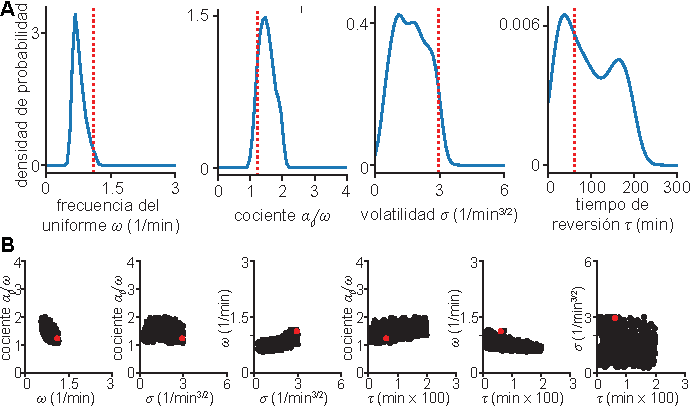
\includegraphics[width=1\columnwidth]{figures/chapter7/C7_OU_fit.pdf} 
    \caption{\textbf{\textit{Posterior} obtenida a partir del Cálculo Bayesiano Aproximado Monte Carlo Secuencial}. (A) Distribuciones marginales. La linea roja punteada indica el parámetro elegido para evaluar el ajuste. (B) Distribuciones marginales combinadas. El punto rojo indica el parámetro elegido para evaluar el ajuste. (A,B) Las distribuciones fueron obtenidas de la \textit{posterior} de los parámetros del modelo de fase de bifurcación de ciclo infinito con la amplitud de modulación como proceso de OU que ajustan a los datos experimentales (figura \ref{C6_fig:observables_experimentales}). Decidimos graficar solamente valores de $\sigma \geq 0$ y $\tau > 0$ porque en este trabajo restringimos nuestro análisis a sólo valores positivos de los parámetros del modelo teórico. Parámetro elegido para evaluar el ajuste: $\omega = 1.11062323539235\; \frac{1}{\text{ min }}$, $\alpha_0 = 1.22764998210094 \times \omega$, $ \sigma = 2.93505385490856 \; \frac{1}{\text{min}^{3/2}}$ y $\tau = 61.0154746022342 \; \text{min} $ (ver apéndice \ref{C7_ap:ABC-SMC}, figura \ref{C7_fig:ap_eps}).}
    \label{C7_fig:OU_fit}
\end{figure} 

%validación
Para continuar, buscamos evaluar la capacidad de este ajuste de reproducir los observables que describen las oscilaciones intermitentes, realizando la misma comparación que en el capítulo anterior (sección \ref{C6_sssec:evaluac_params}). Los valores de $(\omega,\alpha_0,\sigma,\tau)$ con los que elegimos trabajar se encuentran indicados en rojo en la figura \ref{C7_fig:OU_fit}. 

%pulsos aislados y consecutivos
Observamos que el modelo es capaz de reproducir correctamente la cantidad de pulsos totales, pero en este caso sobrestima los consecutivos y subestima los aislados (figura \ref{C7_fig:OU_param_evaluation}A). Esta diferencia se traduce en sistemáticamente una mayor cantidad de trenes de pulsos que nuestras observaciones experimentales (figura \ref{C7_fig:OU_param_evaluation}B).


\begin{figure}
    \centering
    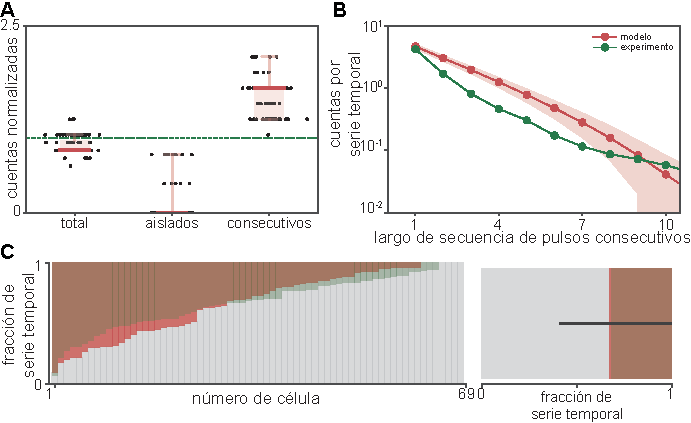
\includegraphics[width=1\columnwidth]{figures/chapter7/C7_OU_validation.pdf} 
    \caption{\textbf{Capacidad del ajuste del ajuste del Cálculo Bayesiano Aproximado Monte Carlo Secuencial para reproducir los observables que describen las oscilaciones intermitentes}. (A)  Mediana de pulsos totales, consecutivos y aislados, normalizados por la mediana de los datos experimentales (puntos negros). Los datos provienen de 100 realizaciones del modelo teórico. Las barras de color representan la mediana, los límites de la caja son los percentiles 25 y 75 de las distribuciones, y los bigotes son los percentiles 5 y 95. La linea verde referencia los valores experimentales. (B) Número de trenes de pulsos en función del número de pulsos consecutivos en el tren para las simulaciones (rojo) y los datos experimentales (verde). El recuento incluye los casos que se producen dentro de trenes más largos, y el primer punto de datos corresponde al número total de pulsos individuales. Los recuentos se han normalizado por el número de series temporales. El área sombreada es desviación estándar de 100 realizaciones independientes del modelo teórico. (C) Izquierda: fracción de tiempo que las series temporales sintéticas individuales pasaron pulsando (rojo) o sin pulsar (gris). A la derecha: Tiempo medio que las series temporales estuvieron pulsando (rojo) o no pulsando (gris). La barra de error indica la desviación estándar calculada sobre la población celular. En verde se indican las mediciones realizadas sobre los experimentos realizados en serum + LIF (capítulo \ref{ch2}). Estas mediciones fueron calculadas sobre 69 series temporales sintéticas de 120 minutos de duración, un conjunto de datos similar al experimental. (A-C) Parámetros: $\omega = \frac{1.11062323539235}{\text{ min }}$, $\alpha_0 = 1.22764998210094 \times \omega$, $ \sigma = 2.93505385490856 \; \frac{1}{\text{min}^{3/2}}$ y $\tau = 61.0154746022342 \text{ min } $ (ver apéndice \ref{C6_ap:ABC-SMC}). La tasa de adquisición fue de $dt = 0.001$, cada $d = 1$ pasos. El umbral de amplitud del algoritmo de detección de pulsos fue $A_{th} = 0.9$, y la distancia umbral fue de $W_{th} = 100\text{ cuadros}$. N = $69$ series temporales. $T = 120$ minutos de duración (figura \ref{C7_fig:OU_traces_VM}).}
    \label{C7_fig:OU_param_evaluation}
\end{figure} 


%actividad
A diferencia del modelo anterior, en la figura \ref{C7_fig:OU_param_evaluation}C observamos que este nuevo modelo puede ajustar correctamente los casos en los que las células únicas pulsaban casi todo el tiempo de medición o no pulsaban, reproduciendo satisfactoriamente la heterogeneidad de nuestras observaciones, al igual que la proporción de tiempo promedio en que las células pulsaban.


Por completitud, los histogramas de la estadística de duración de pulsos, intervalo de interpulsado y tasa de pulsado se encuentran en la figura \ref{C7_fig:OU_param_evaluation_hist}. En el caso de la duración de pulsos, obtuvimos en promedio duraciones más cortas que los experimentos, pero con algunas duraciones más largas. Para los intervalos de interpulsado, pudimos satisfactoriamente reproducir su asimetría característica, pero trasladada hacia valores menores. El haber logrado reproducir esta asimetría probablemente esté relacionado a reproducir la actividad heterogénea experimental. Que la distancia entre el primer cuartil y la media sea notoriamente más pequeña que en los experimentos está posiblemente asociado a más frecuencia de trenes de pulsos de mayor longitud en las series temporales sintéticas. Además, que los intervalos de interpulsado sean en general más cortos puede estar correlacionado con tener menores duraciones de los pulsos. Finalmente, en la tasa de pulsado vemos que hay más células que no pulsan que en los experimentos, efecto que también se puede observar en el panel de la izquierda la figura \ref{C7_fig:OU_param_evaluation}C. Sin embargo, se observa una distribución menos definida que la del capítulo anterior, más parecida a la experimental y reflejando, una vez más, la heterogeneidad de actividad pulsátil. 

\begin{figure}
    \centering
    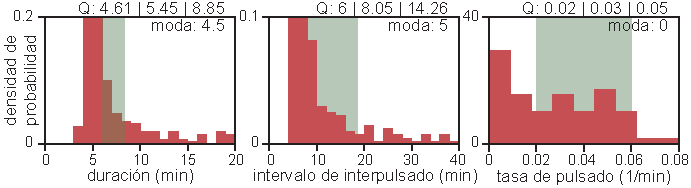
\includegraphics[width=1\columnwidth]{figures/chapter7/C7_OU_validation_hist.pdf} 
    \caption{\textbf{Distribuciones de duración de pulsos, intervalo de interpulsado y tasa de pulsado del ajuste del Cálculo Bayesiano Aproximado Monte Carlo Secuencial}. (A) Distribuciones de la duración de pulsos, el intervalo de interpulsado y la tasa de pulsado, calculadas sobre 69 series temporales sintéticas de 120 minutos de duración, un conjunto de datos similar al experimental. Las unidades del eje $y$ son (1/min), (1/min) y min respectivamente. N = 69 células, $n_1$ = 275 pulsos, $n_2$ = 213 pares de pulsos. Los cuartiles (Q) 25, 50 y 75 y la moda se indican en la parte superior de cada gráfico. Fueron excluidos de los histogramas 27 (duración), 12 (intervalo de interpulsado) y 4 (tasa de pulsado) puntos mayores que el límite del eje x. En verde se indica el rango intercuartílico $IQ$ correspondiente a los experimentos realizados en serum + LIF (figura \ref{C6_fig:observables_experimentales}). Parámetros: $\omega = 1.11062323539235 \; \frac{1}{\text{ min }}$, $\alpha_0 = 1.22764998210094 \times \omega$, $ \sigma = 2.93505385490856 \; \frac{1}{\text{min}^{3/2}}$ y $\tau = 61.0154746022342 \text{ min } $ (ver apéndice \ref{C7_ap:ABC-SMC}). La tasa de adquisición fue de $dt = 0.001$, cada $d = 1$ pasos. El umbral de amplitud del algoritmo de detección de pulsos fue $A_{th} = 0.9$, y la distancia umbral fue de $W_{th} = 100\text{ cuadros}$. N = $69$ series temporales. $T = 120$ minutos de duración (figura \ref{C7_fig:OU_traces_VM}).}
    \label{C7_fig:OU_param_evaluation_hist}
\end{figure} 


En definitiva, incorporar variabilidad en la amplitud de modulación definiéndola como un proceso de OU conduce a reproducir satisfactoriamente la actividad pulsátil heterogénea que observamos en las series temporales de actividad de ERK. Sin embargo, contrariamente al caso considerado en el capítulo anterior, este modelo teórico subestima la cantidad de pulsos consecutivos del experimento y subestima los aislados, conduciendo a una frecuencia más alta de trenes de pulsos largos. Esto demuestra que generar transiciones entre el régimen oscilatorio- produciendo oscilaciones- y el excitable-produciendo intervalos de silencio- es suficiente para reproducir trenes de pulsos largos, pero no para describir los pulsos aislados, reforzando la idea de que estos pulsos aislados son signos de excitabilidad. 


\section{Pulsos aislados como perturbaciones del régimen excitable}
\label{C7_sec:OUD}
%0) motivacion para proponer ESTE nuevo modelo (excitabilidad)


En el capítulo anterior analizamos que es improbable que la actividad pulsátil de ERK provenga únicamente de perturbar de manera sistemática el sistema en el régimen excitable el modelo de fase de bifurcación de ciclo infinito. En ese caso, se tiende a sobrestimar la cantidad de pulsos aislados o en trenes cortos para obtener la misma cantidad de pulsos que en el experimento. En la sección anterior observamos que transiciones entre el régimen excitable y el oscilatorio generadas a partir de introducir variabilidad en la amplitud de modulación son también insuficientes para describir las oscilaciones intermitentes. En este otro caso se tiende a sobrestimar la cantidad de trenes de pulsos y subestimar los pulsos aislados. 

Estos resultados sostienen la idea de que los trenes de pulsos que observamos reflejen actividad oscilatoria de ERK, y los pulsos aislados sean reminiscencias de excitabilidad. Es posible que simultáneamente el sistema dinámico esté transicionando entre un régimen dinámico oscilatorio y un excitable, y a la vez haya perturbaciones que potencialmente darán lugar a actividad pulsátil en el excitable. En esta sección desarrollamos esta idea.


\subsection{Ruido blanco gaussiano aditivo y la amplitud de modulación como proceso de \textit{ornstein-uhlenbeck}}

Para evaluar la posibilidad de que la dinámica de actividad de ERK sea producto de transiciones entre dos régimenes dinámicos y simultáneamente perturbaciones capaz de generar actividad pulsátil en el régimen excitable proponemos estudiar el modelo de fase con bifurcación de ciclo infinito con dos modificaciones: (i) con la amplitud de modulación como un proceso de \textit{Ornstein-Uhlenbeck}, y (ii) con ruido blanco gaussiano aditivo
\begin{equation}
    \partial_t  \theta(t) = \omega + \alpha_{ou}(t) \sin{(\theta(t))} + \sqrt{2D} \xi_w(t).
    \label{C7_eq:alpha_ou_D}
\end{equation}
Con esta descripción, esperamos que el ruido de OU $\alpha_{ou}(t)$ nos conduzca a tener transiciones entre los dos regímenes dinámicos. Durante estas transiciones, el ruido blanco gaussiano aditivo $\sqrt{2D} \xi_w(t)$ tenderá a desordenar las oscilaciones en el régimen oscilatorio, y a la promover la actividad pulsátil en el régimen excitable. 

%PONER SERIES TEMPORALES A MODO DE EJEMPLO CITE 

\subsection{Capacidades y limitaciones para describir las oscilaciones intermitentes de actividad de ERK}

%2) Ajuste
Para evaluar la capacidad del modelo, implementamos el ABC-SMC para obtener una distribución de probabilidad \textit{posterior} de los posibles $(\omega,\alpha_0,\sigma,\tau,D)$ que ajusten a nuestros datos experimentales. Utilizamos la misma implementación y criterios que en la sección \ref{C6_sssec:implementac_ABCSMC}. Las especificaciones de esta implementación se encuentran en el apéndice \ref{C7_ap:ABC-SMC}.


\begin{figure}
    \centering
    \includegraphics[width=1\columnwidth]{figures/chapter7/C7_OUD_fit.pdf} 
    \caption{\textbf{\textit{Posterior} obtenida a partir del Cálculo Bayesiano Aproximado Monte Carlo Secuencial}. (A) Distribuciones marginales. La linea roja punteada indica el parámetro elegido para evaluar el ajuste. (B) Distribuciones marginales combinadas. La barra de color indica la densidad de probabilidad, y el punto rojo indica el parámetro elegido para evaluar el ajuste. (A,B) Las distribuciones fueron obtenidas de la \textit{posterior} de los parámetros del modelo de fase de bifurcación de ciclo infinito con la amplitud de modulación como proceso de OU que ajustan a los datos experimentales (figura \ref{C6_fig:observables_experimentales}). Decidimos graficar solamente valores de $\frac{\alpha_0}{\omega} \geq 0$ , $\sigma  \geq 0$, $\tau  > 0$ y $D  \geq 0$ porque en este trabajo restringimos nuestro análisis sólo en valores positivos de los parámetros del modelo teórico. Parámetro elegido para evaluar el ajuste: $\omega = 0.650550354855668 \; \frac{1}{\text{ min }}$, $\alpha_0 = 1.07946000664919 \times \omega$, $ \sigma = 0.453496764315301 \; \frac{1}{\text{min}^{3/2}}$, $\tau = 142.06010981909 \; \text{min} $ y $D = 0.114054011283622 \; \frac{1}{\text{min}^{2}}$ (ver apéndice \ref{C7_ap:ABC-SMC}, figura \ref{C7_fig:ap_eps}).}
    \label{C7_fig:OUD_fit}
\end{figure} 


En la figura \ref{C7_fig:OUD_fit} podemos observar que las distribuciones marginales obtenidas son unimodales y con un ancho definido.
La distribución marginal de $\alpha_0/\omega$ tiene una moda es cercana a al valor unidad, al igual que en el caso anterior. La volatilidad toma valores más grandes, y el tiempo de reversión consiste en escalas temporales más largas en comparación con el ajuste previo. En este caso la distribución del tiempo de correlación tiene un sólo máximo. Esto sugiere que en el caso anterior las dos escalas temporales modales que observamos posiblemente provengan de intentar describir simultáneamente dos regímenes distintos de pulsado. Por otro lado, la distribución marginal de la intensidad del ruido está bien definida, y toma valores más pequeños comparado con el capítulo anterior. Es posible que esta diferencia consista en que en este modelo el rol del ruido sea principalmente perturbar el régimen excitable, y no competir con el modelo determinista para dominar la dinámica. 


Buscamos evaluar la capacidad de este ajuste de reproducir los observables que describen las oscilaciones intermitentes, realizando la misma comparación que en el capítulo anterior (sección \ref{C6_sssec:evaluac_params}). Los valores de $(\omega,\alpha_0,\sigma,\tau,D)$ con los que elegimos trabajar en esta sección se encuentran indicados en rojo en la figura \ref{C7_fig:OUD_fit}. 

%pulsos aislados y consecutivos
Observamos que el modelo reproduce correctamente la cantidad de pulsos totales y aislados, y en promedio subestima levemente los consecutivos (figura \ref{C7_fig:OUD_param_evaluation}A). Este resultado se condice con la cantidad de trenes de pulsos de determinada duración, donde observamos que las simulaciones reproducen satisfactoriamente la tendencia del comportamiento, incluso hasta la frecuencia de trenes largos de hasta $8$ pulsos (figura \ref{C7_fig:OUD_param_evaluation}B). Además, este modelo ajusta correctamente los casos en los que las células únicas pulsaban casi todo el tiempo de medición o no pulsaban, y reproduce satisfactoriamente tanto la heterogeneidad de nuestras observaciones, como la proporción de tiempo en que las células pulsaban en promedio (figura \ref{C7_fig:OUD_param_evaluation}C). La leve diferencia  entre el modelo y los experimentos en los valores altos de actividad de células únicas posiblemente esté asociado a la presencia de trenes de $9$ o más pulsos, así como la leve subestimación de la cantidad de pulsos consecutivos. 


\begin{figure}
    \centering
    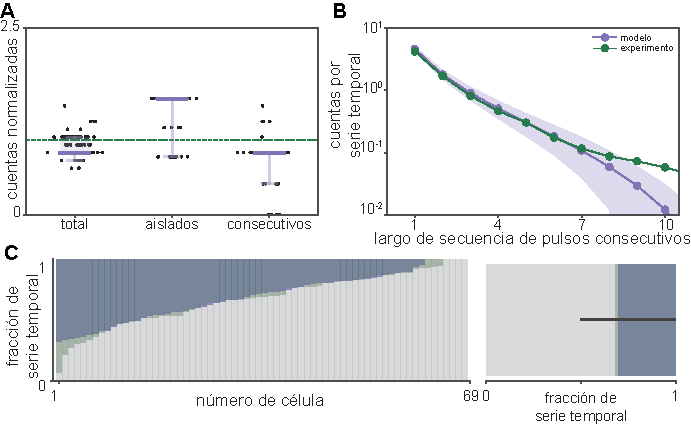
\includegraphics[width=1\columnwidth]{figures/chapter7/C7_OUD_validation.pdf} 
    \caption{\textbf{Capacidad del ajuste del ajuste del Cálculo Bayesiano Aproximado Monte Carlo Secuencial para reproducir los observables que describen las oscilaciones intermitentes}. (A)  Mediana de pulsos totales, consecutivos y aislados, normalizados por la mediana de los datos experimentales (puntos negros). Los datos provienen de 100 realizaciones del modelo teórico. Las barras de color representan la mediana, los límites de la caja son los percentiles 25 y 75 de las distribuciones, y los bigotes son los percentiles 5 y 95. La linea verde referencia los valores experimentales. (B) Número de trenes de pulsos en función del número de pulsos consecutivos en el tren para las simulaciones (violeta) y los datos experimentales (verde). El recuento incluye los casos que se producen dentro de trenes más largos, y el primer punto de datos corresponde al número total de pulsos individuales. Los recuentos se han normalizado por el número de series temporales. El área sombreada es desviación estándar de 100 realizaciones independientes del modelo teórico. (C) Izquierda: fracción de tiempo que las series temporales sintéticas individuales pasaron pulsando (violeta) o sin pulsar (gris). A la derecha: Tiempo medio que las series temporales estuvieron pulsando (violeta) o no pulsando (gris). La barra de error indica la desviación estándar medida sobre la población celular. En verde se indican las mediciones realizadas sobre los experimentos realizados en serum + LIF (capítulo \ref{ch2}). Estas mediciones fueron calculadas sobre 69 series temporales sintéticas de 120 minutos de duración, un conjunto de datos similar al experimental. (A-C) Parámetros:  $\omega = 0.650550354855668 \; \frac{1}{\text{ min }}$, $\alpha_0 = 1.07946000664919 \times \omega$, $ \sigma = 0.453496764315301 \; \frac{1}{\text{min}^{3/2}}$, $\tau = 142.06010981909 \; \text{min} $ y $D = 0.114054011283622 \; \frac{1}{\text{min}^{2}}$ (ver apéndice \ref{C7_ap:ABC-SMC}). La tasa de adquisición fue de $dt = 0.001$, cada $d = 1$ pasos. El umbral de amplitud del algoritmo de detección de pulsos fue $A_{th} = 0.9$, y la distancia umbral fue de $W_{th} = 100\text{ cuadros}$. N = $69$ series temporales. $T = 120$ minutos de duración (figura \ref{C7_fig:OUD_traces_VM}).}
    \label{C7_fig:OUD_param_evaluation}
\end{figure} 


Por completitud, los histogramas de la estadística de duración de pulsos, intervalo de interpulsado y tasa de pulsado se encuentran en la figura \ref{C7_fig:OUD_param_evaluation_hist}. Observamos que la estadística de duración de pulsos se ajusta razonablemente, tantos sus estadísticos como su forma. En el caso de la distribución de intervalo de interpulsado, pudimos también reproducir sus estadísticos. Además, logramos ajustar la forma de la distribución, aunque su cola fue levemente más corta en el ajuste. Posiblemente esta discrepancia esté correlacionada con la leve diferencia que observamos en la figura \ref{C7_fig:OUD_param_evaluation}C, donde se ve que en las simulaciones hay más células sin actividad pulsátil que en los experimentos. En la distribución de tasa de pulsado podemos ver que esta diferencia es más pequeña que en el caso de la sección anterior, donde el modelo no tenía ruido blanco aditivo. 


\begin{figure}
    \centering
    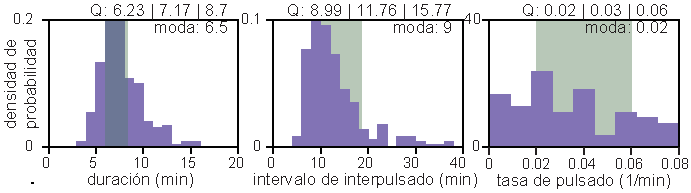
\includegraphics[width=1\columnwidth]{figures/chapter7/C7_OUD_validation_hist.pdf} 
    \caption{\textbf{Distribuciones de duración de pulsos, intervalo de interpulsado y tasa de pulsado del ajuste del Cálculo Bayesiano Aproximado Monte Carlo Secuencial}. (A) Distribuciones de la duración de pulsos, el intervalo de interpulsado y la tasa de pulsado, calculadas sobre 69 series temporales sintéticas de 120 minutos de duración, un conjunto de datos similar al experimental.Las unidades del eje $y$ son (1/min), (1/min) y min respectivamente. N = 69 células, $n_1$ = 333 pulsos, $n_2$ = 271 pares de pulsos. Los cuartiles (Q) 25, 50 y 75 y la moda se indican en la parte superior de cada gráfico. Fueron excluidos de los histogramas 15 (intervalo de interpulsado) y 7 (tasa de pulsado) puntos mayores que el límite del eje x. En verde se indica el rango intercuartílico $IQ$ correspondiente a los experimentos realizados en serum + LIF (figura \ref{C6_fig:observables_experimentales}). Parámetros:  $\omega = 0.650550354855668 \; \frac{1}{\text{ min }}$, $\alpha_0 = 1.07946000664919 \times \omega$, $ \sigma = 0.453496764315301 \; \frac{1}{\text{min}^{3/2}}$, $\tau = 142.06010981909 \; \text{min} $ y $D = 0.114054011283622 \; \frac{1}{\text{min}^{2}}$ (ver apéndice \ref{C7_ap:ABC-SMC}). La tasa de adquisición fue de $dt = 0.001$, cada $d = 1$ pasos. El umbral de amplitud del algoritmo de detección de pulsos fue $A_{th} = 0.9$, y la distancia umbral fue de $W_{th} = 100\text{ cuadros}$. N = $69$ series temporales. $T = 120$ minutos de duración (figura \ref{C7_fig:OUD_traces_VM}).}
    \label{C7_fig:OUD_param_evaluation_hist}
\end{figure} 


En resumen, tener simultáneamente transiciones entre el régimen oscilatorio y el excitable, y ruido blanco gaussiano aditivo capaz de generar actividad pulsátil en el régimen excitable es capaz de producir intervalos oscilatorios intercalados con intervalos de silencios y pulsos aislados. Con estos resultados, creemos que este modelo teórico es suficiente para describir las principales características dinámicas de las oscilaciones intermitentes de ERK en ESCs. Además, encontramos que es posible generar oscilaciones intermitentes con escalas temporales similares a las que medimos en los experimentos. 


Observamos en la figura \ref{C7_fig:OUD_fit}A que existen tiempos de retorno largos en los resultados del ajuste, que son comparables con la duración de nuestras mediciones experimentales de aproximadamente 2 horas. Con estos tiempos de retorno, es posible que el sistema dinámico se encuentre en un sólo régimen dinámico durante toda la medición y se pueda considerar a la amplitud de modulación como estacionaria. En estos hipotéticos casos en donde la amplitud de modulación es estacionaria, podríamos prescindir de incorporar una escala temporal para representar su variabilidad. En la próxima sección desarrollamos esta idea.


\section{Variabilidad en la amplitud de modulación como proceso estacionario}
\sectionmark{Amplitud de modulación como proceso estacionario}
\label{C7_sec:dist}

%motivación
Observamos que en el modelo anterior el ajuste arrojó tiempos de retorno comparables con la duración de nuestras mediciones experimentales de aproximadamente dos horas (figura \ref{C7_fig:OUD_fit}). Este resultado sugiere la posibilidad de que la variabilidad que representamos en la amplitud de modulación pueda ser estacionaria. Con esta hipótesis, la amplitud de modulación tomaría un valor fijo constante, y en principio distinto para cada célula. 


\subsection{Distribución gaussiana de muestreo de la amplitud de modulación}
\subsectionmark{Distribución gaussiana de la amplitud de modulación}

Consideraremos el modelo de fase de bifurcación de ciclo infinito y ruido blanco gaussiano aditivo
\begin{equation}
    \partial_t  \theta_i(t) = \omega + \alpha_i \sin{(\theta_i(t))}+ \sqrt{2D} \xi_w(t),
\end{equation}
en donde $i$ es el índice celular. Con esta descripción, cada medición tendrá una amplitud de modulación $\alpha_i$ fija y, en principio, diferente. Además, cada medición de una célula $i$ tendrá una trayectoria propia $\theta_i(t)$. 


Describir a cada célula con un valor distinto de la amplitud de modulación implica que cada una de las trayectorias del sistema dinámico tenga la posibilidad de estar en un régimen dinámico diferente. En los casos en donde $\alpha_i < \omega$, las trayectorias de la fase serán oscilatorias, y el ruido destruirá la coherencia de las oscilaciones. Cuando $\alpha_i > \omega$, el sistema estará en el régimen excitable, y existe la posibilidad de que el ruido perturbe al sistema y genere actividad pulsátil. Proponemos adquirir a la amplitud de modulación de una distribución gaussiana de media $\mu_{\alpha}$ y desviación estándar $\sigma_{\alpha}$ en cada medición. Como en este trabajo asumimos que la amplitud de modulación es semipositiva, truncamos en cero esta distribución (figura \ref{C7_fig:dist_def}).


\begin{figure}
    \centering
    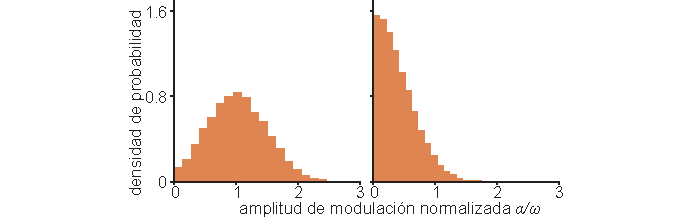
\includegraphics[width=1\columnwidth]{figures/chapter7/C7_dist_def.pdf} 
    \caption{\textbf{Distribución de muestreo de la amplitud de modulación.} Posibles distribuciones de muestreo gaussianas truncadas de la amplitud de modulación. Izquierda: $\mu_{\alpha} = 1 \; \frac{1}{\text{min}}$. Derecha: $\mu_{\alpha} = 0$. En ambos casos $\sigma_{\alpha} = 0.5 \; \frac{1}{\text{min}}$ y N = 10000. }
    \label{C7_fig:dist_def}
\end{figure} 


\subsection{Capacidades y limitaciones para describir las oscilaciones intermitentes de actividad de ERK}

%2) Ajuste
Para evaluar la capacidad del modelo, implementamos el ABC-SMC para obtener una distribución de probabilidad \textit{posterior} de los posibles $(\omega,\mu_{\alpha},\sigma_{\alpha},D)$ que ajusten a nuestros datos experimentales. Utilizamos la misma implementación y criterios que en la sección \ref{C6_sssec:implementac_ABCSMC}. Las especificaciones de esta implementación se encuentran en el apéndice \ref{C7_ap:ABC-SMC}.


\begin{figure}
    \centering
    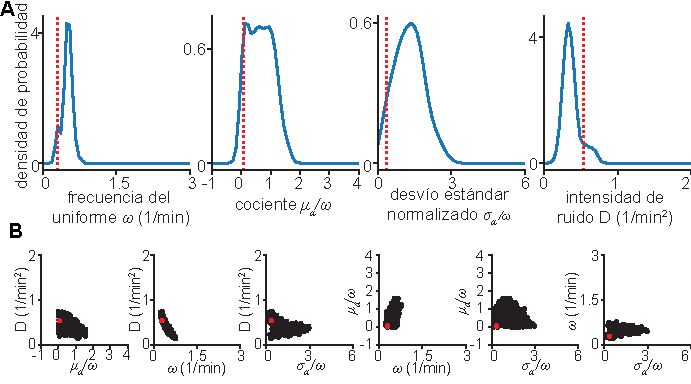
\includegraphics[width=1\columnwidth]{figures/chapter7/C7_dist_fit.pdf} 
    \caption{\textbf{\textit{Posterior} obtenida a partir del Cálculo Bayesiano Aproximado Monte Carlo Secuencial}. (A) Distribuciones marginales. La linea roja punteada indica el parámetro elegido para evaluar el ajuste. (B) Distribuciones marginales combinadas. El punto rojo indica el parámetro elegido para evaluar el ajuste. (A,B) Las distribuciones fueron obtenidas de la \textit{posterior} de los parámetros del modelo de fase de bifurcación de ciclo infinito con la amplitud de modulación como proceso de OU que ajustan a los datos experimentales (figura \ref{C6_fig:observables_experimentales}). Decidimos graficar solamente valores de $\sigma_{\alpha}  > 0$ porque definimos el desvío estándar positivo. Parámetro elegido para evaluar el ajuste: $\omega = 0.298471928449595 \; \frac{1}{\text{ min }}$, $\mu_{\alpha} = 0.0646569119807585 \times \omega$, $ \sigma_{\alpha} = 0.358175275333557 \;  \times \omega $ y $D = 0.541442551452375 \; \frac{1}{\text{min}^{2}}$ (ver apéndice \ref{C7_ap:ABC-SMC}, figura \ref{C7_fig:ap_eps}).}
    \label{C7_fig:dist_fit}
\end{figure} 


En la figura \ref{C7_fig:dist_fit}A podemos observar que las distribuciones marginales obtenidas son unimodales y con un ancho definido. En particular, la distribución marginal del valor medio de la distribución de muestreo de la amplitud de modulación normalizado por la frecuencia del uniforme estaba centrada en uno, y la del desvío estándar normalizado presentaba valores comparables. En la figura \ref{C7_fig:dist_fit}B observamos una anticorrelación entre estas dos distribuciones marginales. Para valores medios pequeños, el ancho de la distribución es más grande, y para valores medios más grandes, la distribución de la amplitud de modulación es más definida. Esto sugiere que para reproducir la estadística de los observables de la dinámica de actividad de ERK, posiblemente sean necesarios valores altos de la amplitud de modulación que conduzcan al régimen excitable, y valores pequeños que lo hagan al oscilatorio.  


Para continuar, buscamos evaluar la capacidad de este ajuste de reproducir los observables que describen las oscilaciones intermitentes, realizando la misma comparación que en el capítulo anterior (sección \ref{C6_sssec:evaluac_params}). Los valores de $(\omega,\mu_{\alpha},\sigma_{\alpha},D)$ con los que elegimos trabajar en esta sección se encuentran indicados en rojo en la figura \ref{C7_fig:dist_fit}. 

\begin{figure}
    \centering
    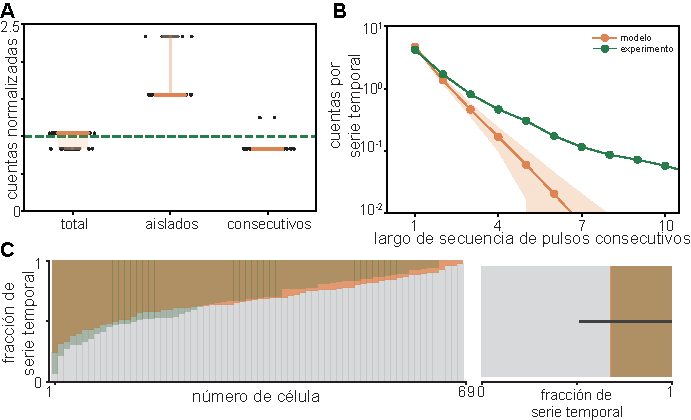
\includegraphics[width=1\columnwidth]{figures/chapter7/C7_dist_validation.pdf} 
    \caption{\textbf{Capacidad del ajuste del ajuste del Cálculo Bayesiano Aproximado Monte Carlo Secuencial para reproducir los observables que describen las oscilaciones intermitentes}. (A)  Mediana de pulsos totales, consecutivos y aislados, normalizados por la mediana de los datos experimentales (puntos negros). Los datos provienen de 100 realizaciones del modelo teórico. Las barras de color representan la mediana, los límites de la caja son los percentiles 25 y 75 de las distribuciones, y los bigotes son los percentiles 5 y 95. La linea verde referencia los valores experimentales. (B) Número de trenes de pulsos en función del número de pulsos consecutivos en el tren para las simulaciones (naranja) y los datos experimentales (verde). El recuento incluye los casos que se producen dentro de trenes más largos, y el primer punto de datos corresponde al número total de pulsos individuales. Los recuentos se han normalizado por el número de series temporales. El área sombreada es desviación estándar de 100 realizaciones independientes del modelo teórico. (C) Izquierda: fracción de tiempo que las series temporales sintéticas individuales pasaron pulsando (naranja) o sin pulsar (gris). A la derecha: Tiempo medio que las series temporales estuvieron pulsando (naranja) o no pulsando (gris). La barra de error indica la desviación estándar calculada sobre la población celular. En verde se indican las mediciones realizadas sobre los experimentos realizados en serum + LIF (capítulo \ref{ch2}). Estas mediciones fueron calculadas sobre 69 series temporales sintéticas de 120 minutos de duración, un conjunto de datos similar al experimental. (A-C) Parámetros:  $\omega = 0.298471928449595 \; \frac{1}{\text{ min }}$, $\mu_{\alpha} = 0.0646569119807585 \times \omega$, $ \sigma_{\alpha} = 0.358175275333557  \times \omega$ y $D = 0.541442551452375 \; \frac{1}{\text{min}^{2}}$ (ver apéndice \ref{C7_ap:ABC-SMC}). La tasa de adquisición fue de $dt = 0.001$, cada $d = 1$ pasos. El umbral de amplitud del algoritmo de detección de pulsos fue $A_{th} = 0.9$, y la distancia umbral fue de $W_{th} = 100\text{ cuadros}$. N = $69$ series temporales. $T = 120$ minutos de duración (figura \ref{C7_fig:dist_traces_VM}).}
    \label{C7_fig:dist_param_evaluation}
\end{figure} 

%pulsos aislados y consecutivos
Observamos en la figura \ref{C7_fig:dist_param_evaluation}A que cuando modelo reproduce correctamente la cantidad de pulsos totales, subestima la cantidad de pulsos consecutivos y sobrestima los aislados. Al igual que en el capítulo anterior, esto conduce a subestimar la frecuencia de trenes de pulsos largos (figura \ref{C7_fig:dist_param_evaluation}B). Sin embargo, es interesante que el modelo reproduce satisfactoriamente la heterogeneidad de nuestras observaciones de actividad (figura \ref{C7_fig:dist_param_evaluation}C). Observamos gran similitud entre la actividad poblacional en el modelo y los experimentos, incluso en los casos en los que las células no pulsan o pulsan a lo largo de casi toda la medición. Como anteriormente, este ajuste se ve acompañado por el ajuste de la actividad media poblacional.


Por completitud, los histogramas de la estadística de duración de pulsos, intervalo de interpulsado y tasa de pulsado se encuentran en la figura \ref{C7_fig:dist_param_evaluation_hist}. Si bien la estadística de duración de pulsos se ajusta razonablemente, su forma demuestra que hay una mayor variabilidad en las duraciones de pulsos del modelo que del experimento. Previamente estudiamos que la duración de pulsos depende de la amplitud de modulación. Estos resultados sugieren que valores altos de desvío estándar de la distribución de muestreo de $\alpha_i$ conduzcan a distribuciones de duración de pulsos anchas.  La variabilidad observada en la distribución de duración de pulsos también se observa en la distribución de intervalos de interpulsado.


\begin{figure}
    \centering
    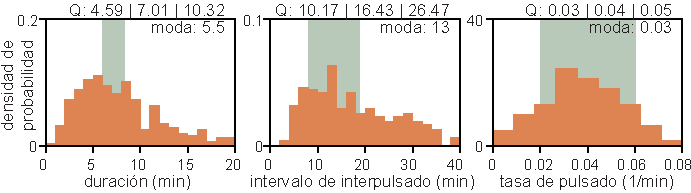
\includegraphics[width=1\columnwidth]{figures/chapter7/C7_dist_validation_hist.pdf} 
    \caption{\textbf{Distribuciones de duración de pulsos, intervalo de interpulsado y tasa de pulsado del ajuste del Cálculo Bayesiano Aproximado Monte Carlo Secuencial}. Distribuciones de la duración de pulsos, el intervalo de interpulsado y la tasa de pulsado, calculadas sobre 69 series temporales sintéticas de 120 minutos de duración, un conjunto de datos similar al experimental. Las unidades del eje $y$ son (1/min), (1/min) y min respectivamente. N = 69 células, $n_1$ = 327 pulsos, $n_2$ = 258 pares de pulsos. Los cuartiles (Q) 25, 50 y 75 y la moda se indican en la parte superior de cada gráfico. Fueron excluidos de los histogramas 9 (duración) y 19 (intervalo de interpulsado) puntos mayores que el límite del eje x. En verde se indica el rango intercuartílico $IQ$ correspondiente a los experimentos realizados en serum + LIF (figura \ref{C6_fig:observables_experimentales}). Parámetros:  $\omega = 0.298471928449595 \; \frac{1}{\text{ min }}$, $\mu_{\alpha} = 0.0646569119807585 \times \omega$, $ \sigma_{\alpha} = 0.358175275333557  \times \omega$ y $D = 0.541442551452375 \; \frac{1}{\text{min}^{2}}$ (ver apéndice \ref{C7_ap:ABC-SMC}). La tasa de adquisición fue de $dt = 0.001$, cada $d = 1$ pasos. El umbral de amplitud del algoritmo de detección de pulsos fue $A_{th} = 0.9$, y la distancia umbral fue de $W_{th} = 100\text{ cuadros}$. N = $69$ series temporales. $T = 120$ minutos de duración (figura \ref{C7_fig:dist_traces_VM}).}
    \label{C7_fig:dist_param_evaluation_hist}
\end{figure} 


Los resultados que obtuvimos nos demuestran que es posible reproducir la heterogeneidad de actividad pulsátil que observamos en los experimentos sin necesidad de asumir una escala temporal que regule la variabilidad de la amplitud de modulación. Sin embargo, cuando analizamos cómo están ordenados los pulsos, encontramos que no es posible describir la estadística de trenes de pulsos largos de observaciones experimentales. Esto sugiere que para reproducir las oscilaciones intermitentes de actividad de ERK en ESCs es necesario incorporar una escala temporal que regule las transiciones del sistema dinámico entre el régimen oscilatorio y el excitable. 


\section{Conclusiones y discusión}

%Rol de ruido en bio. Posibles fuentes de ruido

Buscamos describir las oscilaciones intermitentes de la dinámica de activación de ERK en ESCs, donde intervalos oscilatorios se intercalan con intervalos de silencio y pulsos aislados. En el capítulo anterior consideramos un modelo de fase con bifurcación de ciclo infinito y ruido blanco gaussiano aditivo, que resultó insuficiente para describir esta dinámica. Principalmente fallaba en recapitular la heterogeneidad de actividad que observamos en los datos experimentales, y en que los pulsos solían ser aislados o estar organizados en trenes cortos en comparación con nuestras observaciones. En este capítulo estudiamos modificaciones de este modelo. 

%OU
Comenzamos por explorar la idea de que la actividad pulsátil de ERK pueda ser descripta a partir de transiciones entre el régimen oscilatorio y el excitable, que sin perturbaciones dará lugar a intervalos de silencio. Incluimos variabilidad en la amplitud de modulación del modelo de fase con bifurcación de ciclo infinito, a partir de definirla como un proceso de \textit{Ornstein-Uhlenbeck} (figura \ref{C7_fig:OU_TS}). 
Implementamos el método de Cálculo Bayesiano Aproximado basado en la implementación de Monte Carlo Secuencial para obtener una distribución de probabilidad \textit{posterior} de los posibles parámetros de esta nueva descripción teórica que ajusten a nuestros datos experimentales (figura  \ref{C7_fig:OU_fit}). A partir de esta calibración, elegimos un grupo de parámetros con el cual evaluar la capacidad del modelo de describir las oscilaciones intermitentes. 

La nueva propuesta fue capaz de recapitular la heterogeneidad de actividad pulsátil de nuestras observaciones, al igual que la proporción de tiempo promedio en que las células pulsaban. La reproducción de esta característica devino en un histograma de tasa de pulsado menos definido y más parecido al del experimento que el analizado en el capítulo anterior, y en una distribución de intervalos de interpulsado de cola larga como la experimental (figura \ref{C7_fig:OU_param_evaluation_hist}). También reprodujo la cantidad de pulsos totales, pero sobrestimaba los consecutivos y subestimaba los aislados (figura \ref{C7_fig:OU_param_evaluation}). Esta diferencia se tradujo en sistemáticamente una mayor cantidad de trenes largos de pulsos que nuestras observaciones experimentales, y en una distribución de intervalos de interpulsado con una distancia entre el primer cuartil y la media más pequeña que en los experimentos. 

Generar transiciones entre el régimen oscilatorio- produciendo oscilaciones- y el excitable-produciendo intervalos de silencio- resultó ser suficiente para reproducir trenes de pulsos largos, pero no para describir los pulsos aislados. Esto refuerza la idea de que estos pulsos aislados son signos de excitabilidad. Que en este modelo los trenes de pulsos estén mayoritariamente organizados en trenes de pulsos consecutivos largos se contrapone con nuestras observaciones del capítulo anterior, donde los pulsos solían ser aislados o estar organizados en trenes cortos. 

%OUD
Consideramos, entonces, un nuevo sistema dinámico que simultáneamente daba lugar a transiciones entre los regímenes dinámicos oscilatorio y excitable, y tenía perturbaciones capaces de generar actividad pulsátil en el excitable. En este sistema, el modelo de fase con bifurcación de ciclo infinito tenía (i) una amplitud de modulación descripta como un proceso de \textit{Ornstein-Uhlenbeck}, y (ii) ruido blanco gaussiano aditivo. A partir de calibrar este nuevo modelo, elegimos un grupo de parámetros con el cual evaluar su capacidad de describir las oscilaciones intermitentes (figura \ref{C7_fig:OUD_fit}).

Encontramos que el modelo reproducía correctamente las principales características que describen las oscilaciones intermitentes (figura \ref{C7_fig:OUD_param_evaluation}). Con esta descripción logramos recapitular la cantidad de pulsos totales y aislados del experimento. La comparación entre este resultado y el primer modelo que consideramos en este capítulo nos sugiere que es necesario excitar el régimen excitable para describir la estadística de pulsos aislados de nuestras observaciones. Además, la moda de la distribución marginal de tiempo de reversión fue más definida y con valores más grandes en este modelo que en el caso anterior (figuras \ref{C7_fig:OU_fit}, \ref{C7_fig:OUD_fit}). En el caso anterior, donde no había excitaciones, el sistema dinámico debía reproducir simultáneamente pulsos aislados y consecutivos, lo que posiblemente condujo a un ajuste de estas características. 


Además, reprodujimos satisfactoriamente la tendencia de la frecuencia de de trenes de pulsos de determinada duración, incluso hasta la frecuencia de trenes largos de hasta 8 pulsos. El contraste de este resultado con el obtenido el capítulo anterior nos indica que es necesario tener transiciones entre el régimen excitable y el oscilatorio para reproducir la estadística de trenes de pulsos largos que adquirimos en los experimentos. 

Este modelo también logró reproducir satisfactoriamente tanto la heterogeneidad de la actividad pulsátil de nuestras observaciones, como la proporción de tiempo en que las células pulsaban en promedio. 

Observamos una leve discrepancia con los experimentos, que detectamos en varios observables. Esta diferencia consistió en subestimar los valores altos de actividad pulsátil de células únicas, la presencia de trenes de 9 o más pulsos, y una leve subestimación de la cantidad de pulsos consecutivos. Tanto en el análisis de trenes de pulsos como en el de actividad pulsátil de células individuales, las regiones en donde el modelo no coincide con las simulaciones son regiones límite en donde la evolución de los datos experimentales parece no responder a la tendencia que se registra en cada análisis. Sustenta esta idea que el modelo sin ruido blanco aditivo considerado previamente sí reproduzca el comportamiento en estas regiones (figura \ref{C7_fig:OU_param_evaluation}). Este cambio de comportamiento de los datos experimentales podría un genuino comportamiento de la actividad dinámica de ERK, o podría ser consecuencia de limitaciones en las mediciones experimentales. Para discriminar entre estas dos opciones, sería conveniente a futuro realizar nuevas mediciones experimentales de igual frecuencia de adquisición, pero más largas. 

En resumen, creemos que este modelo es suficiente para describir las principales características dinámicas de las oscilaciones intermitentes de ERK en ESCs. Incluso es posible generar oscilaciones intermitentes con escalas temporales similares a las que medimos en los experimentos (figura \ref{C7_fig:OUD_param_evaluation_hist}). 

%DIST
El ajuste de este modelo arrojó tiempos de retorno que regulan la variabilidad en la amplitud de modulación comparables con la duración de nuestras mediciones experimentales (figura \ref{C7_fig:OUD_fit}). Este resultado nos condujo a evaluar si la variabilidad en la amplitud de modulación podía ser descripta como un proceso estacionario, y no un proceso que varíe durante cada medición como hipotetizamos en los dos casos anteriores.  Para esto, consideramos un nuevo modelo de fase de bifurcación de ciclo infinito. En este caso, agregamos ruido blanco gaussiano aditivo, y cada medición tenía una amplitud de modulación positiva muestreada de una distribución gaussiana. A partir de calibrar este nuevo modelo, elegimos un grupo de parámetros con el cual evaluar su capacidad de describir las oscilaciones intermitentes (figura \ref{C7_fig:dist_fit}).

Encontramos que cuando el modelo reproducía correctamente la cantidad de pulsos totales, podía simultáneamente recapitular de manera satisfactoria la heterogeneidad de nuestras observaciones de actividad pulsátil, así como la promedio. Esto nos indica que es posible reproducir la heterogeneidad de actividad pulsátil que observamos en los experimentos sin necesidad de asumir una escala temporal que regule la variabilidad de la amplitud de modulación. Este resultado es consistente con lo propuesto en sección \ref{C2_sec:pulsado_estoctastico}, donde desarrollamos la idea de que la heterogeneidad en la actividad pulsátil que observamos tenga origen en una heterogeneidad propia celular.


Por otro lado, previamente estudiamos que la duración de pulsos depende de la amplitud de modulación. Estos resultados sugieren que valores altos de desvío estándar de la distribución de muestreo de la amplitud de modulación conduzcan a distribuciones de duración de pulsos anchas, como la que observamos en este caso (figura \ref{C7_fig:dist_param_evaluation_hist}). 

Por último, el modelo subestimaba la cantidad de pulsos consecutivos y sobrestimaba los aislados, subestimando también la frecuencia de trenes de pulsos largos (figura \ref{C7_fig:dist_param_evaluation}). Esto sugiere que para reproducir las oscilaciones intermitentes de actividad de ERK en ESCs es necesario incorporar una escala temporal que regule las transiciones del sistema dinámico entre los régimenes oscilatorio y el excitable. 


En resumen, encontramos que es posible describir las oscilaciones intermitentes de actividad de ERK en ESCs con un modelo matemático minimalista con algunos ingredientes. Como base, tenemos un modelo de fase de bifurcación de ciclo infinito determinista que puede lugar a dos regímenes dinámicos: uno oscilatorio y uno excitable. Luego, describir a la amplitud de modulación como un proceso de OU permite tener transiciones gobernadas por una escala temporal entre estos dos regímenes, que posiblemente den lugar a los intervalos oscilatorios intercalados con intervalos de silencios. Por otro lado, incorpora variabilidad en la amplitud de modulación, responsable de la heterogeneidad poblacional de la actividad pulsátil. Finalmente, incluir ruido blanco gaussiano aditivo genera excitaciones en el régimen excitable, y conduce a la posibilidad de tener pulsos aislados. 


A partir de estas observaciones, se abren algunos interrogantes. Por ejemplo, ¿de qué parámetros depende la longitud de los intervalos oscilatorios, o la tasa de pulsado?, o ¿es posible variar estas cantidades pero mantener la duración de pulsos constante? Responder este tipo de preguntas es clave para describir cómo depende la dinámica de activación de ERK de FGF en ESCs, y entender cómo la red de transducción de señales FGF/ERK codifica información importante para las decisiones de destino celular. 


Para responder a estas preguntas, creemos necesario perfeccionar el protocolo con el que ajustamos los parámetros del modelo. Estas mejoras podrían significar dar con una nueva definición de distancia en la implementación del ABC-SMC. De esta manera, podríamos lograr que el ABC-SMC ajuste no sólo a los rangos intercuartílicos de las distribuciones de duración de pulsos, intervalo de interpulsado y tasa de pulsado, sino también a la forma de las distribuciones. Podríamos también proponer ajustar otras medidas más complejas, como por ejemplo la cantidad de trenes de pulsos de una determinada longitud. Estas mejoras también podrían ser efectuar mediciones de la estadística de series temporales más largas durante cada iteración del ABC-SMC. 

En paralelo, el algoritmo de detección de pulsos utilizado en este capítulo fue diseñado para el modelo de fase de bifurcación de ciclo infinito y ruido blanco gaussiano del capítulo anterior. Si bien funciona satisfactoriamente, en los modelos de fase con la amplitud de modulación como proceso de OU de las secciones \ref{C7_sec:OU} y \ref{C7_sec:OUD} consideramos a los puntos fijos como los correspondientes al valor medio de la amplitud de modulación para implementar la detección (apéndice \ref{C7_ap:OU_OUD_traces}). Probablemente este criterio conduzca a impresiones en la detección del inicio y el final de un pulso, y en consecuencia a impresiones en las mediciones de duración de pulsos. Como el comportamiento de la distribución de duración de pulsos está correlacionado con la de intervalos de interpulsado, estas imprecisiones son fáciles de detectar. Sin embargo, mejorar estas mediciones posiblemente conduzca a medir la duración de pulsos de manera más precisa, y mejores resultados. 



\begin{subappendices}
\section{Simulaciones numéricas de series temporales y detección de pulsos}
\label{C7_ap:OU_OUD_traces}

Para generar numéricamente las trayectorias de la amplitud de modulación como proceso de \textit{Ornstein-Uhlenbeck}, implementamos el algoritmo de Heun de \cite{SanMiguel2000}. Para generar las trayectorias de la fase en donde la amplitud de modulación incorpora ruido de color, tanto en la sección \ref{C7_sec:OU} como en \ref{C7_sec:OUD} donde incorporamos ruido blanco aditivo, utilizamos el método de Runge-Kutta que implementa ideas similares al método de Heun descripto en \cite{SanMiguel2000}. Este enfoque es un poco más costoso computacionalmente, pero tiene la ventaja converger correctamente al ruido blanco gaussiano para valores pequeños de tiempo de retorno. Para generar números aleatorios utilizamos el método de Box-Muller-Wiener. 


Generamos las series temporales $x(t)$ con un paso o frecuencia de sampleo de $dt$ por un total de $T$ minutos, y $n = T/dt $ pasos. Adquirimos puntos de la trayectoria de $x(t)$ cada $d$ pasos. Por lo general, las condiciones iniciales fueron sampleadas de una distribución uniforme $U(0,2\pi)$, al menos que se indique lo contrario. En el caso de la amplitud de modulación, la condición inicial fue su valor medio $\alpha_0$.

Para detectar pulsos, utilizamos el algoritmo descripto en el capítulo anterior (sección \ref{C6_ssec:deteccion_de_pulsos}). En los modelos de fase con la amplitud de modulación como proceso de OU de las secciones \ref{C7_sec:OU} y \ref{C7_sec:OUD}, consideramos a los puntos fijos como los correspondientes al valor medio de la amplitud de modulación $\alpha_0$.



\section{Especificaciones de la implementación del ABC-SMC}
\label{C7_ap:ABC-SMC}

Como \textit{prior} propusimos la siguiente distribución uniforme
\begin{equation*}
    \Pi(x) = \left\{ \begin{array}{lcc}
             \frac{1}{b-a} &   \text{si}  & x \in [a,b] \\
             \\ 0 &  \text{si} & x < a \; \text{o} \; x > b.
             \end{array}
   \right.
\end{equation*}
Los límites $a$ y $b$ de cada uno de los parámetros fueron elegidos previa inspección visual del sistema dinámico. Una correcta elección de estas funciones agiliza la convergencia del algoritmo, siendo posible que durante las iteraciones se recorran parámetros que inicialmente no están contemplados en estas \textit{prior}. 

En la sección \ref{C7_sec:OU}, para la frecuencia del uniforme $\omega$, $a = \frac{\pi}{14 \text{ min}}$ y $b = \frac{8\pi}{7 \text{ min}}$. Para el cociente adimensional $\alpha_0/\omega$, $a = 0$ y $b = 2$. Para el tiempo de reversión $\tau$, $a = 1$ y $b = 200$ minutos, y para la volatilidad $\sigma$, $a = 0$ y $b = 3$ $\frac{1}{\text{min}^{3/2}}$. 

En la sección \ref{C7_sec:OUD}, para la frecuencia del uniforme $\omega$, $a = \frac{\pi}{14 \text{ min}}$ y $b = \frac{8\pi}{7 \text{ min}}$. Para el cociente adimensional $\alpha_0/\omega$, $a = 0$ y $b = 2$. Para el tiempo de reversión $\tau$, $a = 1$ y $b = 200$ minutos. Para la volatilidad $\sigma$, $a = 0$ y $b = 3$ $\frac{1}{\text{min}^{3/2}}$, y para la intensidad de ruido $D$, $a = 0$ y $b = 2\;\frac{1}{\text{min}^2}$.

En la sección \ref{C7_sec:dist}, para la frecuencia del uniforme $\omega$, $a = \frac{\pi}{14 \text{ min}}$ y $b = \frac{8\pi}{7 \text{ min}}$. Para el cociente adimensional $\alpha_0/\omega$, $a = 0$ y $b = 2$. Para la desviación estándar normalizada $\sigma_{\alpha}/\omega$, $a = 0$ y $b = 5$, y para la intensidad de ruido $D$, $a = 0$ y $b = 2\;\frac{1}{\text{min}^2}$.


En las secciones \ref{C7_sec:OU} y \ref{C7_sec:OUD} cada serie temporal simulada durante la implementación del algoritmo tenía una frecuencia de sampleo $dt = 0.001 \text{ min}$, una frecuencia de adquisición de $d = 1$ paso y una duración total de $T = 1000 \text{ min}$. Para calcular la distribución de duración de pulsos de cada serie temporal, utilizamos el algoritmo de detección de pulsos descripto en la sección \ref{C6_ssec:deteccion_de_pulsos}, con un umbral de amplitud $A_{th} = 0.9$ y una distancia umbral $W_{th} = 100 \text{ cuadros}$. También utilizamos el resultado de implementar este algoritmo para estimar la la mediana de la tasa de pulsado como cantidad de pulsos detectados sobre $T = 1000 \text{ min}$. Para obtener la distribución de intervalo de interpulsado, utilizamos el procedimiento descripto en la sección \ref{C6_ssec:deteccion_de_pulsos}.  


En la sección \ref{C7_sec:dist} cada serie temporal simulada durante la implementación del algoritmo tenía una frecuencia de sampleo $dt = 0.001 \text{ min}$, una frecuencia de adquisición de $d = 1$ paso y una duración total de $T = 100 \text{ min}$. En cada evaluación simulamos $30$ series temporales con estas características, cada una con una amplitud de modulación distinta que adquirimos de distribución de muestreo definida por los parámetros $\mu_{\alpha}$ y $\sigma_{\alpha}$. Para calcular la distribución de duración de pulsos de cada serie temporal, utilizamos el algoritmo de detección de pulsos descripto en la sección \ref{C6_ssec:deteccion_de_pulsos}, con un umbral de amplitud $A_{th} = 0.9$ y una distancia umbral $W_{th} = 100 \text{ cuadros}$ para cada una de las 30 series temporales.  Para obtener la distribución de intervalo de interpulsado,  utilizamos el procedimiento descripto en la sección \ref{C6_ssec:deteccion_de_pulsos} para cada serie temporal. Finalmente, para calculamos la tasa de pulsado de cada serie temporal, y luego tomamos su mediana. 


Durante todo este capítulo, la tolerancia mínima que determinaba el final del algoritmo fue de $\epsilon = 0.1$, que elegimos basándonos en la implementación de \cite{Costa2021}. También establecimos un número máximo de $21$ iteraciones, límite al cual no fue necesario recurrir. Las tolerancias que obtuvimos en cada una de las implementaciones se encuentran en la figura 
\ref{C7_fig:ap_eps}.

\begin{figure}
    \centering
    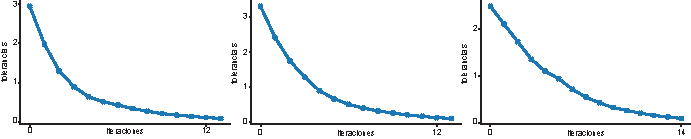
\includegraphics[width=1\columnwidth]{figures/chapter7/C7_eps.pdf} 
    \caption{\textbf{Convergencia del Cálculo Bayesiano Aproximado Monte Carlo Secuencial}. Evolución de la tolerancia a medida que aumentan las iteraciones para el modelo de las secciones \ref{C7_sec:OU} (izquierda),  \ref{C7_sec:OUD} (centro) y  \ref{C7_sec:dist} (derecha).}
    \label{C7_fig:ap_eps}
\end{figure} 


Los 1000 parámetros aceptados por el ABC-SMC y sus respectivos pesos se encuentran en \href{https://github.com/fiorefabris/parameters}{el este \underline{link}}. En casa caso, se encuentra marcado en rojo los parámetros que utilizamos para ejemplificar los resultados de cada ajuste. 


Las series temporales surgidas del conjunto de parámetros que elegimos para validar el modelo, así como el resultado del algoritmo de detección de pulsos se encuentran en las figuras \ref{C7_fig:OU_traces_VM} (sección \ref{C7_sec:OU}), \ref{C7_fig:OUD_traces_VM} (sección \ref{C7_sec:OUD}) y \ref{C7_fig:dist_traces_VM} (sección \ref{C7_sec:dist}) . Decidimos en este caso visualizar las series temporales a partir del observable 
\begin{equation}
    X(t) = \frac{e^{k\sin{(\theta(t))}}}{e^{k}},
    \label{C7_eq:VM}
\end{equation}
donde elegimos k = 100. Con esta transformación, es más sencillo distinguir a simple vista las excursiones de la fase del ruido de fondo. Esta ventaja es en detrimento de (i) utilizar una expresión más compleja que la de la ecuación \ref{C5_eq:seno_fase}, y (ii) que las excursiones de la fase en sentido horario, que en este trabajo no consideramos como pulsos, también son más fáciles de distinguir a simple vista y más difíciles de distinguir de las excursiones en sentido antihorario, o pulsos. 


\begin{figure}
    \centering
    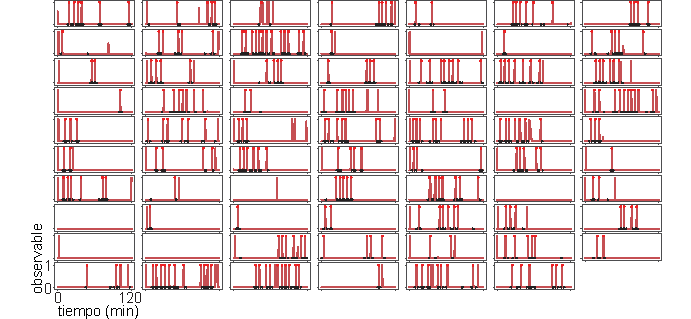
\includegraphics[width=1\columnwidth]{figures/chapter7/C7_OU_traces_for_evaluation_VM.pdf} 
    \caption{\textbf{Series temporales sintéticas y detección de pulsos para explorar el modelo de fase con bifurcación de ciclo infinito y amplitud de modulación como proceso de \textit{Ornstein-Uhlenbeck}.} Series temporales del observable \ref{C7_eq:VM} de la fase en función del tiempo para el modelo de la sección \ref{C7_sec:OU}. Se encuentra también representado el resultado del algoritmo de detección de pulsos, donde el inicio (triángulo negro con el vértice del lado izquierdo), el pico (rojo) y el final (triángulo negro con el vértice del lado derecho) de cada pulso detectado están indicados. Los picos observados que no fueron identificados como pulsos son, en su mayoría, excursiones de la fase en sentido horario. Parámetros: $\omega = 1.11062323539235\; \frac{1}{\text{ min }}$, $\alpha_0 = 1.22764998210094 \times \omega$, $ \sigma = 2.93505385490856 \; \frac{1}{\text{min}^{3/2}}$ y $\tau = 61.0154746022342 \; \text{min} $. La tasa de adquisición fue de $dt$ = $0.001$, cada $d = 1$ pasos. El umbral de amplitud del algoritmo de detección de pulsos fue $A_{th} = 0.9$, y la distancia umbral fue de $W_{th} = 100\text{ cuadros}$. N = $69$ series temporales. $T = 120$ minutos de duración.}
    \label{C7_fig:OU_traces_VM}
\end{figure}

 
\begin{figure}
    \centering
    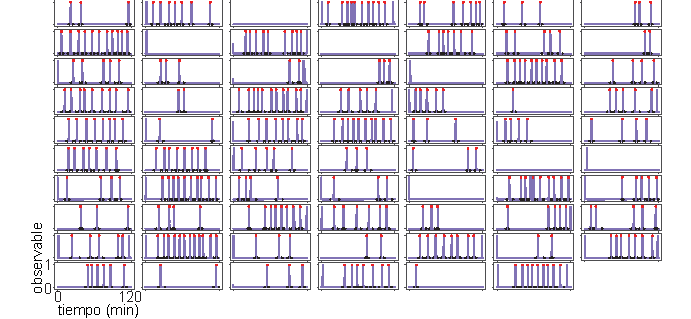
\includegraphics[width=1\columnwidth]{figures/chapter7/C7_OUD_traces_for_evaluation_VM.pdf} 
    \caption{\textbf{Series temporales sintéticas y detección de pulsos para explorar el modelo de fase con bifurcación de ciclo infinito, amplitud de modulación como proceso de \textit{Ornstein-Uhlenbeck} y ruido blanco gaussiano aditivo.} Series temporales del observable \ref{C7_eq:VM} de la fase en función del tiempo para el modelo de la sección \ref{C7_sec:OUD}. Se encuentra también representado el resultado del algoritmo de detección de pulsos, donde el inicio (triángulo negro con el vértice del lado izquierdo), el pico (rojo) y el final (triángulo negro con el vértice del lado derecho) de cada pulso detectado están indicados. Los picos observados que no fueron identificados como pulsos son, en su mayoría, excursiones de la fase en sentido horario. Parámetros: $\omega = 0.650550354855668 \; \frac{1}{\text{ min }}$, $\alpha_0 = 1.07946000664919 \times \omega$, $ \sigma = 0.453496764315301 \; \frac{1}{\text{min}^{3/2}}$, $\tau = 142.06010981909 \; \text{min} $ y $D = 0.114054011283622 \; \frac{1}{\text{min}^{2}}$. La tasa de adquisición fue de $dt$ = $0.001$, cada $d = 1$ pasos. El umbral de amplitud del algoritmo de detección de pulsos fue $A_{th} = 0.9$, y la distancia umbral fue de $W_{th} = 100\text{ cuadros}$. N = $69$ series temporales. $T = 120$ minutos de duración.}
    \label{C7_fig:OUD_traces_VM}
\end{figure}

\begin{figure}
    \centering
    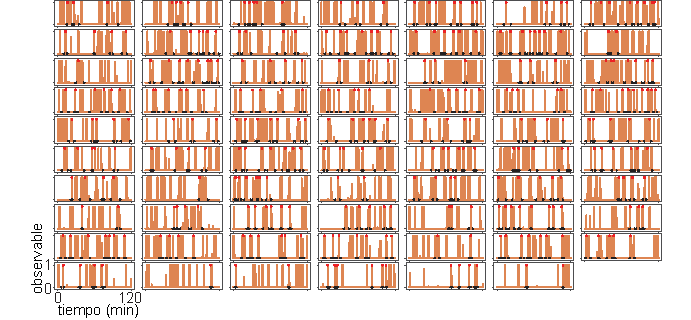
\includegraphics[width=1\columnwidth]{figures/chapter7/C7_dist_traces_for_evaluation_VM.pdf} 
    \caption{\textbf{Series temporales sintéticas y detección de pulsos para explorar el modelo de fase con bifurcación de ciclo infinito, ruido blanco gaussiano aditivo y variabilidad en la amplitud de modulación estacionaria.} Series temporales del observable \ref{C7_eq:VM} de la fase en función del tiempo para el modelo de la sección \ref{C7_sec:OUD}. Se encuentra también representado el resultado del algoritmo de detección de pulsos, donde el inicio (triángulo negro con el vértice del lado izquierdo), el pico (rojo) y el final (triángulo negro con el vértice del lado derecho) de cada pulso detectado están indicados. Los picos observados que no fueron identificados como pulsos son, en su mayoría, excursiones de la fase en sentido horario. Parámetros: $\omega = 0.298471928449595 \; \frac{1}{\text{ min }}$, $\mu_{\alpha} = 0.0646569119807585 \times \omega$, $ \sigma_{\alpha} = 0.358175275333557  \times \omega$ y $D = 0.541442551452375 \; \frac{1}{\text{min}^{2}}$. La tasa de adquisición fue de $dt$ = $0.001$, cada $d = 1$ pasos. El umbral de amplitud del algoritmo de detección de pulsos fue $A_{th} = 0.9$, y la distancia umbral fue de $W_{th} = 100\text{ cuadros}$. N = $69$ series temporales. $T = 120$ minutos de duración.}
    \label{C7_fig:dist_traces_VM}
\end{figure}

\end{subappendices}







\begin{comment}
Formalmente, la correlación de la amplitud de modulación en los casos anteriores depende de el tiempo de reversión $\tau$, y la volatilidad $\sigma^2$. Cuando el tiempo de reversión es grande comparado con nuestras mediciones, podemos suponer que $\tau \rightarrow \infty$. En este límite,

\begin{align}
    \lim_{\tau \to +\infty} \langle \alpha(t) \; \alpha(t^\prime) \rangle_t &=\lim_{\tau \to +\infty} \sigma^2 e^{- \lvert t-t^\prime \rvert / \tau }\\
    &= \sigma^2 \delta_{t\; t^\prime}.
\end{align}


Si tomamos el límite también en la ecuación \ref{C7_eq:OU_langevin},
\begin{align}
     \lim_{\tau \to +\infty} \partial_t  \alpha(t) &=  \lim_{\tau \to +\infty} \big(\frac{1}{\tau} (\alpha_0 - \alpha(t)) + \sqrt{\frac{2}{\tau}}\sigma \xi_w(t) \big) \\
        &= 0,
\end{align}
y el valor de la amplitud de modulación (así como su valor medio) va a estar dado por su condición inicial 
\begin{equation}
    \alpha(t) &= \alpha_0.
\end{equation}
Con estos resultados, podemos asumir 

\end{comment}

\end{document}